% !TeX root = ../sustechthesis-example.tex

\chapter[简介]{简介\label{section:introduction}}
\section[量子计算和量子测控]{量子计算和量子测控}
\subsection[量子计算]{量子计算}
量子计算因其强大的计算能力和潜在的应用前景而受到广泛关注。
在量子算法的配合下,量子计算机可以实现许多通过经典计算机难以实现的计算,如大素数分解\cite[]{Shor_1997, Singleton_Jr_2023}、量子多体系统仿真\cite[]{Feynman_1982, Lloyd_1996}、加速搜索过程\cite[]{Grover_2002}等。

和经典计算机的实现方式类似,量子计算机也采用\emph{比特(Bit)}作为计算单元来实现计算。与经典计算机使用的\emph{经典比特(Bit)}不同的是量子计算的计算单元是\emph{量子比特(Qubit)}。在量子计算机中,这个最小的计算单元通常被表示为:$\ket{0}$和$\ket{1}$。经典比特可能处于的状态只有两个,一般来说$0$(低电平)或$1$(高电平),而量子比特不仅可能处于$\ket{0}$态或$\ket{1}$态,还可能处于两者的概率叠加状态。采用\emph{狄拉克符号(Dirac-Notation)}的方式,一个量子比特可以被表示为概率叠加:$$\ket{\phi}=a_0\ket{0}+a_1\ket{1}$$

其中$a_0^2+a_1^2=1$。对于多个量子比特共同存在的情况,整个系统$(N-qubits)$的状态可以被表示为:$$\ket{\phi}=a_0\ket{0\dots0}+\dots+a_{2^N-1}\ket{1\dots1}$$

这就是所谓的\emph{量子叠加原理(Principle of Quantum Superposition, PQS)}\cite[]{Fedorov_Manko_2019}。这也是量子计算机的\emph{量子并行性(Quantum Parallelism)}这一强大特性的来源。

为了实现量子比特,量子计算机的最小计算单元,我们必须有某种定义明确的两级系统,并且对要编码的信息具有量子效应。David DiVincenzo对量子计算机的实现要素进行了总结\cite[]{DiVincenzo_2000}:
\begin{enumerate}
    \item 一个定义明确的两级系统来编码量子比特;
    \item 足够长的相干时间来执行量子操作;
    \item 能够将量子比特近乎完美的初始化到确定性纯态;
    \item 定义的量子比特能够组合实现通用量子门;
    \item 接近完美的量子比特状态读出;
\end{enumerate}

以上的这些原则被用于选择合适的物理平台来进行量子计算的实现,经过筛选后目前已经被证明有实现通用量子计算机潜力的物理系统平台有:离子阱系统、超导系统、线性光学系统、硅基量子点、原子系统、拓扑系统等。

迄今为止,作为1995年提出的量子计算的第一个候选者的激光冷却\emph{离子阱系统(Ion trap system)}仍然是实现大规模量子计算机最有前途的平台之一。离子已经很好地定义了具有极长相干时间\cite[]{Fisk_Sellars_Lawn_Coles_1997}的内部状态,它保证了出色的纠缠和初始化特性\cite[]{Blatt_Wineland_2008}。储存在单个离子中的的量子比特状态可以有长达几秒钟的寿命\cite[]{Langer_Ozeri_Jost_Chiaverini_DeMarco_Ben_Kish_Blakestad_Britton_Hume_Itano_et_al_2005},在\emph{动态解耦技术(Dynamic Decoupling Technology, DCT)}的帮助下这个寿命可以超过$10$分钟\cite[]{Wang_Um_Zhang_An_Lyu_Zhang_Duan_Yum_Kim_2017},这是在所有现有量子计算物理平台中保持最长的相干时间记录。关于纠缠态的制备,离子阱系统在2011年已经实现了$14$个纠缠态的制备\cite[]{Monz_Schindler_Barreiro_Chwalla_Nigg_Coish_Harlander_Hänsel_Hennrich_Blatt_2011},这个数字在2018年更新到了20\cite[]{Friis_Marty_Maier_Hempel_Holzäpfel_Jurcevic_Plenio_Huber_Roos_Blatt_et_al_2018}。同时,四量子比特多部纠缠态的存储时间达到$1.1$秒\cite[]{Kaufmann_Ruster_Schmiegelow_Luda_Kaushal_Schulz_von_Lindenfels_Schmidt_Kaler_Poschinger_2017}。
此外,运动自由度可以用于实现不同量子位之间的通信,确保全量子位连接\cite[]{Debnath_Linke_Figgatt_Landsman_Wright_Monroe_2016}。离子的状态也可以用几乎完美的效率读出\cite[]{Myerson_Szwer_Webster_Allcock_Curtis_Imreh_Sherman_Stacey_Steane_Lucas_2008},在此基础上可以构建高保真量子逻辑门\cite[]{Ballance_Harty_Linke_Sepiol_Lucas_2016}。
DiVincenzo的原始论文还为量子通信目的指定了两个额外的标准:能平稳地进行量子比特和所谓的“飞行”量子比特之间的相互转换(这可能是光子,量子信息编码在偏振、频率或相位),以及将这些飞行量子比特从一个位置高保真地传输到另一个位置的能力。如果目标不是构建一个平稳的大规模量子计算机,这些标准并不重要,但对于包括量子网络在内的其它一些应用来说是十分必要的。在这方面,一些方案采用捕获离子的中尺度模块之间的光子互连来实现量子处理器的互联\cite[]{Monroe_Raussendorf_Ruthven_Brown_Maunz_Duan_Kim_2014}。虽然离子本身不太可能作为长距离量子通信或量子网络的飞行量子比特,但离子和光子之间的高保真纠缠已被实现\cite[]{Moehring_Blinov_Madsen_Duan_Monroe_2004}。
总之,离子满足QC的五个主要DiVincenzo标准,也验证了将它们的量子信息转移到飞行量子比特的能力。事实上,早在2004,所有这些标准在离子量子比特平台基本上都得到满足\cite[]{Leibfried_DeMarco_Meyer_Lucas_Barrett_Britton_Itano_Jelenković_Langer_Rosenband_et_al_2003,Moehring_Blinov_Madsen_Duan_Monroe_2004}。

尽管到目前为止离子阱量子计算发展迅速,但在实现通用量子计算机之前仍有许多问题有待解决。最近,许多研究这致力于芯片离子阱\cite[]{Mehta_Eltony_Bruzewicz_Chuang_Ram_Sage_Chiaverini_2014}、离子穿梭和规模化\cite[]{Monroe_Kim_2013, Sterling_Rattanasonti_Weidt_Lake_Srinivasan_Webster_Kraft_Hensinger_2014, Lee_Jeong_Park_Jung_Kim_Cho_2021}、光学集成\cite[]{Niffenegger_Stuart_Sorace_Agaskar_Kharas_Bramhavar_Bruzewicz_Loh_Maxson_McConnell_Reens_et_al_2020, Mehta_Zhang_Malinowski_Nguyen_Stadler_Home_2020}、多离子的单独寻址\cite[]{Ivory_Setzer_Karl_McGuinness_DeRose_Blain_Stick_Gehl_Parazzoli_2020}和量子比特纠错\cite[]{Cramer_Kalb_Rol_Hensen_Blok_Markham_Twitchen_Hanson_Taminiau_2016,Reichardt_2021}等技术,以实现最终目标——\emph{通用量子计算机(Universal Quantum Computer, UQC)}。

\subsection[量子测控]{量子测控}

\begin{figure}
    \centering
    \caption[离子阱量子计算的组成]{离子阱量子计算的四大组成部分\label{fig:quantum_computing_ion_trap_system}}
    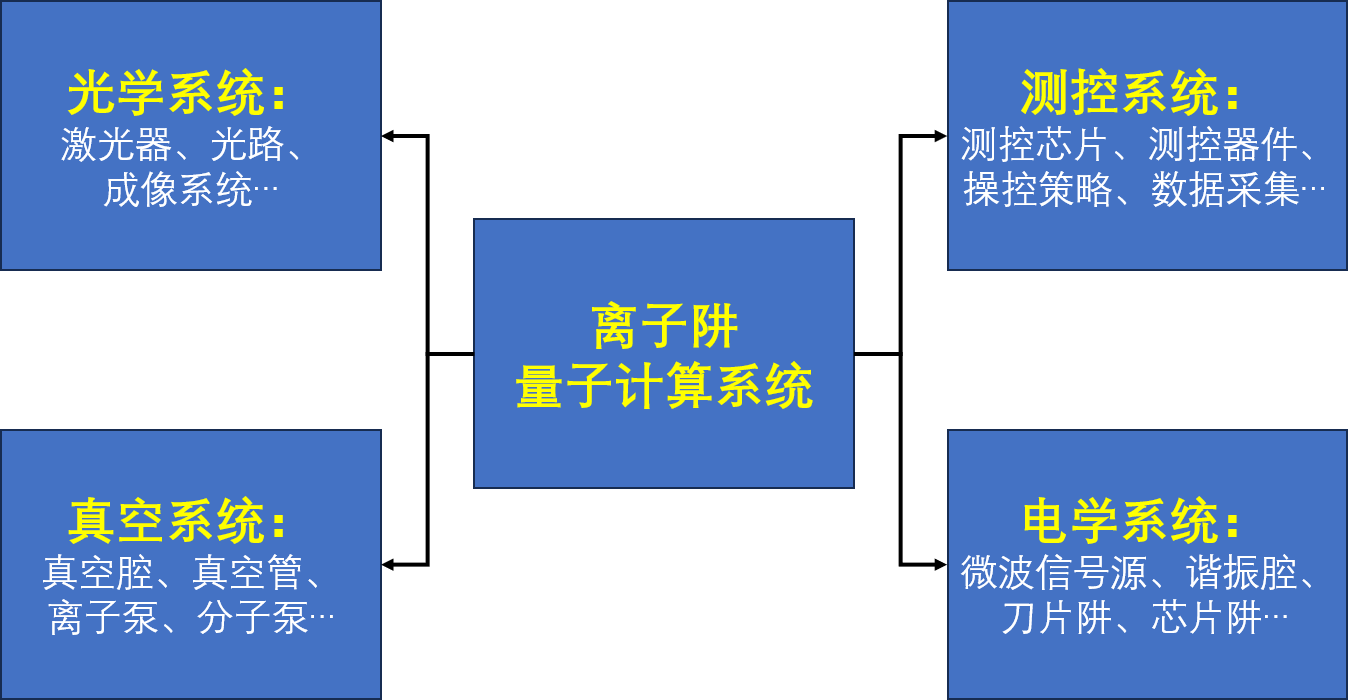
\includegraphics[width=0.8\linewidth]{quantum_computing_ion_trap_system}
\end{figure}
离子阱量子计算系统是一个复杂综合的系统,如图\ref{fig:quantum_computing_ion_trap_system}所示,它主要由四大部分组成:1.  电学系统,主要包括微波信号源、谐振腔、刀片阱、芯片阱等;2. 光学系统,主要包括激光器、由各类镜片组成的光路、成像系统等;3. 真空系统,主要包括真空腔、真空管、离子泵、分子泵等;4. 测控系统,主要包括测控芯片、测控器件、操控策略、数据采集等。想要实现基于离子阱的量子计算需要以上各大部分的相互配合。其中量子测控系统处于十分核心的地位,它将电学、光学、真空等其余各个部分联系了起来,给出特定的微波信号、激光信号等策略对量子比特进行调控并采集结果进行分析和处理。

量子物理实验常常涉及到一些物理量的精确调控和测量,这既包括量上的精确性,也包括时间上的精确性。随着量子技术的发展,量子物理实验系统也开始产生对数据处理、复杂流程控制和实时控制的需求。不同于传统行业,量子物理实验系统对时间控制的精度和分辨率的要求在纳秒量级、延迟要求在百纳秒至数十微秒量级,与当前微处理器的主频相当,这对量子物理实现的测控系统提出了很多新的要求。

\section[论文章节结构介绍]{论文章节结构介绍}
% \textcolor{red}{简要阐述一下后续章节的主要内容...}
离子量子计算是当前最具发展前景的量子计算平台之一,它的实现需要电子、光学、真空、测控等多种学科领域的支持。其中测控系统扮演着至关重要的角色,测控系统涵盖着十分广阔的范围,包括测控核心板卡以及由其构成的如结合螺线管谐振腔的离子阱频率稳定、结合激光器的激光功率和激光拍频稳定等相关测控子系统。本文主旨为面向离子阱量子计算的实验测控系统研究,主要的研究成果和贡献如下:1. 提出了一种强实时性、拓展性好、高度数字化和集成化的RTMQ量子测控系统架构,并且实现了与之匹配高速通用数字PID和高速通用数字滤波器;2. 针对离子囚禁系统中的重要器件——螺线管谐振腔,以更高的Q值和更稳定易用的设计为目标进行了仿真、实验、建模、设计等方面的优化研究;3. 在此基础之上,基于RTMQ测控板卡搭建并测试了离子量子计算系统中几个关键的子系统:离子阱频率稳定系统、激光功率稳定系统和激光拍频稳定系统,为实现集成化、数字化、低成本、灵活稳定的离子量子计算系统奠定了基础。

以面向离子阱量子计算的实验测控系统研究为引领,本论文后续的章节结构如下:
\begin{itemize}
    \item 第\ref{section:quantum_computation}章,作为研究的基础和背景,介绍囚禁离子量子比特的相关内容。包括离子囚禁和量子化过程中涉及的在囚禁势场中的经典和量子运动,离子运动的量子化和离子与光场的耦合,离子(具体来说是镱离子)作为量子比特的编码和操控方案以及基于离子的通用量子门的构建;
    \item 第\ref{section:fpga_rtmq}章,提出了一种强实时性、拓展性好、高度数字化和集成化的量子测控系统架构——RTMQ,展示了它的架构和板卡实现。同时介绍了与之相匹配的高速通用数字PID和高速通用数字滤波器的设计实现,这两个模块儿的实现和集成是RTMQ的重要片上拓展,使得RTMQ测控系统板卡具备更强的适用性;
    \item 第\ref{section:helical}章,针对螺线管谐振腔这种离子囚禁系统中的重要测控器件进行了仿真、实验、建模、设计等方面的优化研究。针对Q值和频率进行了仿真模型的建立并与实验制作测量结果进行了验证,谐振腔更高的Q值可以提高离子囚禁的稳定性和离子比特的保真度。同时,针对旧有谐振腔惯用设计的机械缺点,给出了一种更加稳定易用、更模块儿化且装配方便的谐振腔机械结构设计;
    \item 第\ref{section:implementation}章,基于第\ref{section:fpga_rtmq}章RTMQ测控系统和第\ref{section:helical}章的内容并结合实际的实验系统需求实现了RTMQ测控系统在离子量子计算应用场景下的几个关键子系统搭建和测试,展示了RTMQ系统的优越性,极大地促进了离子量子计算系统的集成化进程,同时也可以满足未来大规模通用量子计算对拓展性的需求;
    \item 最后一章,对本论文进行了总结并对离子量子计算及量子测控领域未来的发展进行了展望。
\end{itemize}